\documentclass{beamer}
%\documentclass[handout]{beamer}

\usepackage[utf-8]{inputenc}
\usepackage[spanish]{babel}
\usepackage{graphicx,verbatim,fancyvrb,array,multirow}

\mode<handout>
{
	\usepackage{pgfpages}
	\pgfpagesuselayout{2 on 1}[a4paper,border shrink=5mm]

	\setbeamercolor{background canvas}{bg=black!0}
	\setbeameroption{show notes}
}

\mode<presentation>
{
	\usetheme{Warsaw}
	\setbeamercovered{transparent}
}

\title{CILA 2006}
\subtitle{Introducción a KDE}

\author[Jonás Regueira Rodríguez y Esaú Rodríguez Sicilia]{
	Jonás Regueira Rodríguez \\
	Esaú Rodríguez Sicilia
}

\begin{document}
\begin{frame}
  \titlepage
\end{frame}
\frame{
	\frametitle{Offtopic}
	\begin{itemize}
		\item Asistencia: 80\% de las clases.
		\item Evaluación: Examen tipo test en la última hora de clase del último día (18-11-06).
		\item Apuntes: http://cila.ssl.ull.es.
		\item Party instalación Bardinux 1 noviembre.
		\item Si no tienes ningún CD Bardinux aprovecha y coge tu copia en el descanso.
	\end{itemize}
}
\section{Entornos de escritorio libres}
\subsection{¿Qué es un escritorio?}
\frame{
	\frametitle{¿Qué es un escritorio?}
	\begin{center}
		
\includegraphics[height=3cm,width=4cm]{./imgs/escritorio.jpg}
	\end{center}
  Conjunto de software que ofrece al usuario un entorno amigable con barras e
iconos con los que lanzar a ejecutar programas.

}

\subsection{GNOME}
\frame
{
	\begin{center}
		Un vistazo rápido a GNOME 2.12
		
\includegraphics[width=8.8cm]{./imgs/gnome-2_12.jpg}
	\end{center}	
}
\subsection{KDE}
\frame
{
	\begin{center}
		Un vistazo rápido a KDE 3.5.2
		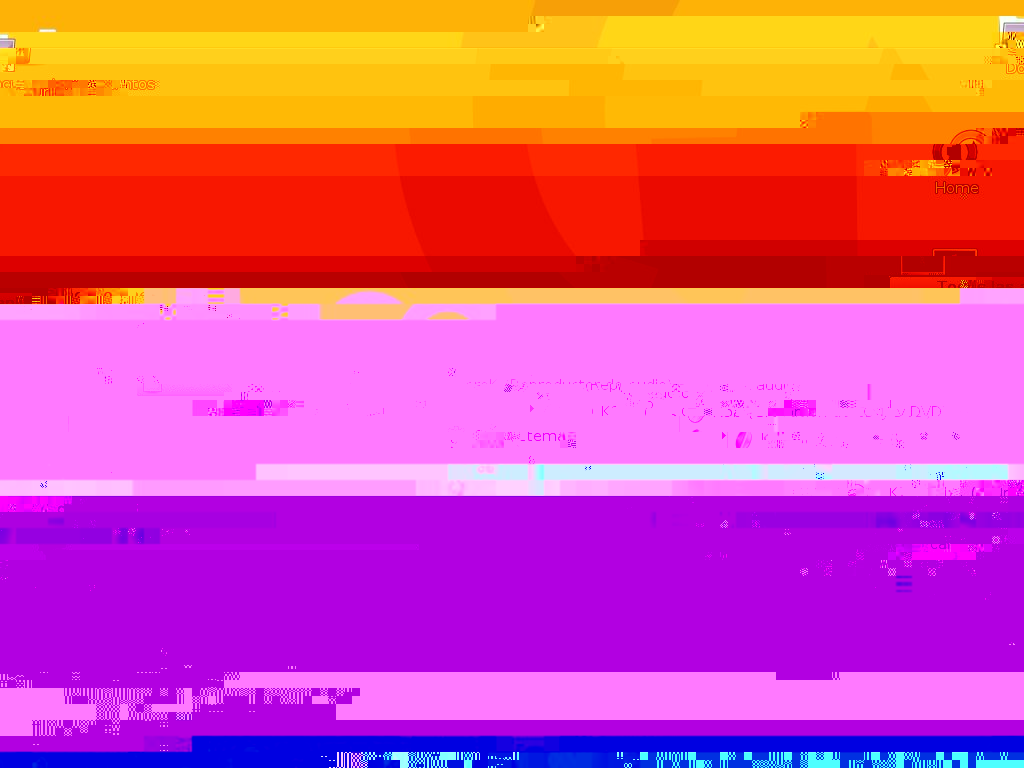
\includegraphics[width=8.8cm]{./imgs/pantallazoBardinux.jpg}
	\end{center}	
}
\subsection{Otros}
\frame
{
	\begin{center}
		\begin{tabular}{cc}
			\begin{tabular}c
		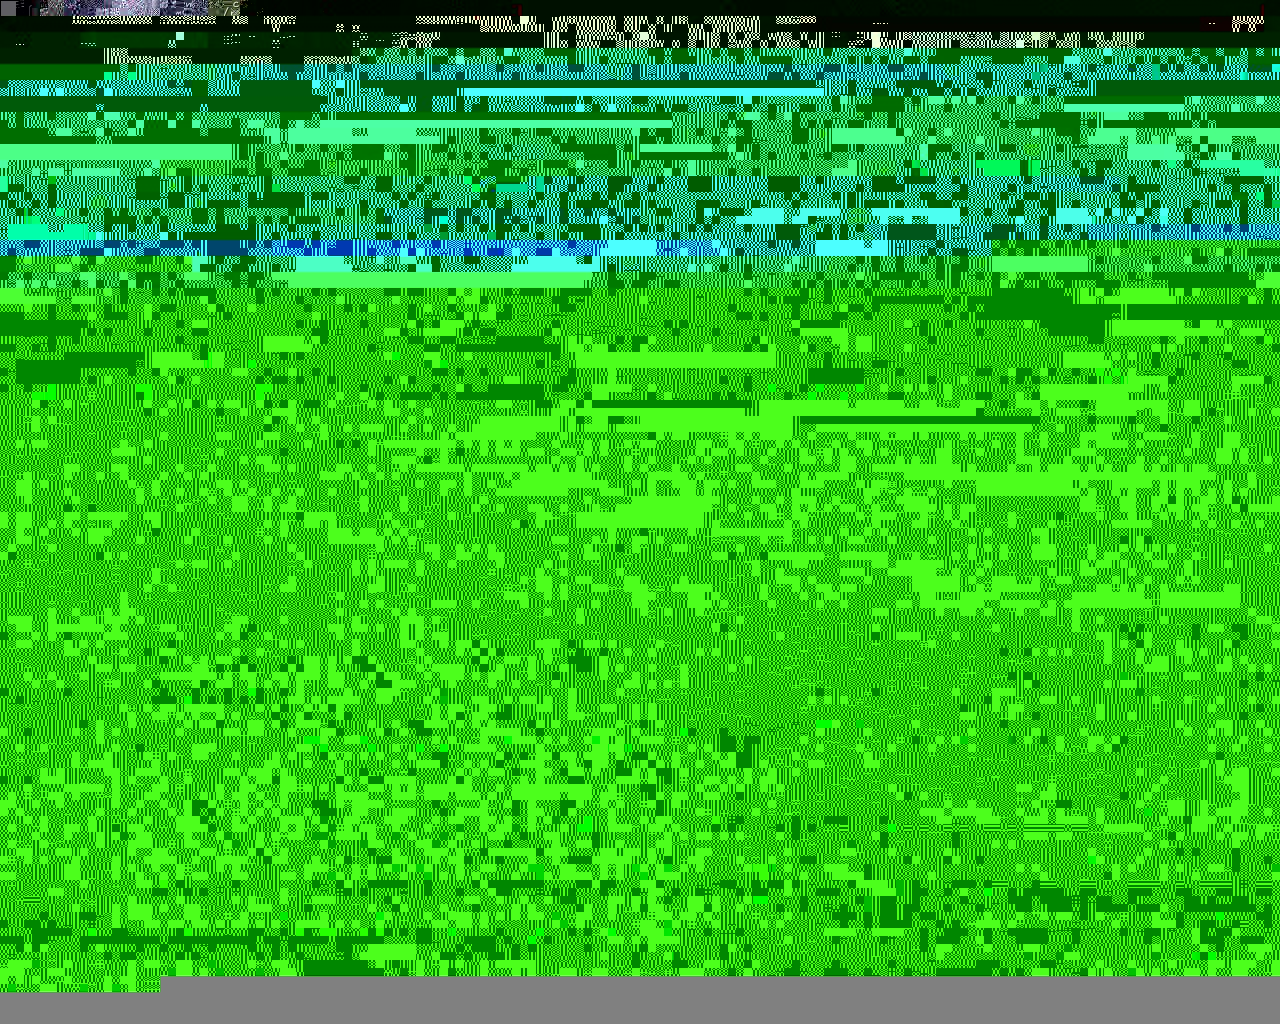
\includegraphics[height=3cm,width=4cm]{./imgs/enlightenment.jpg} \\ Enlightenment
			\end{tabular} &
			\begin{tabular}c
		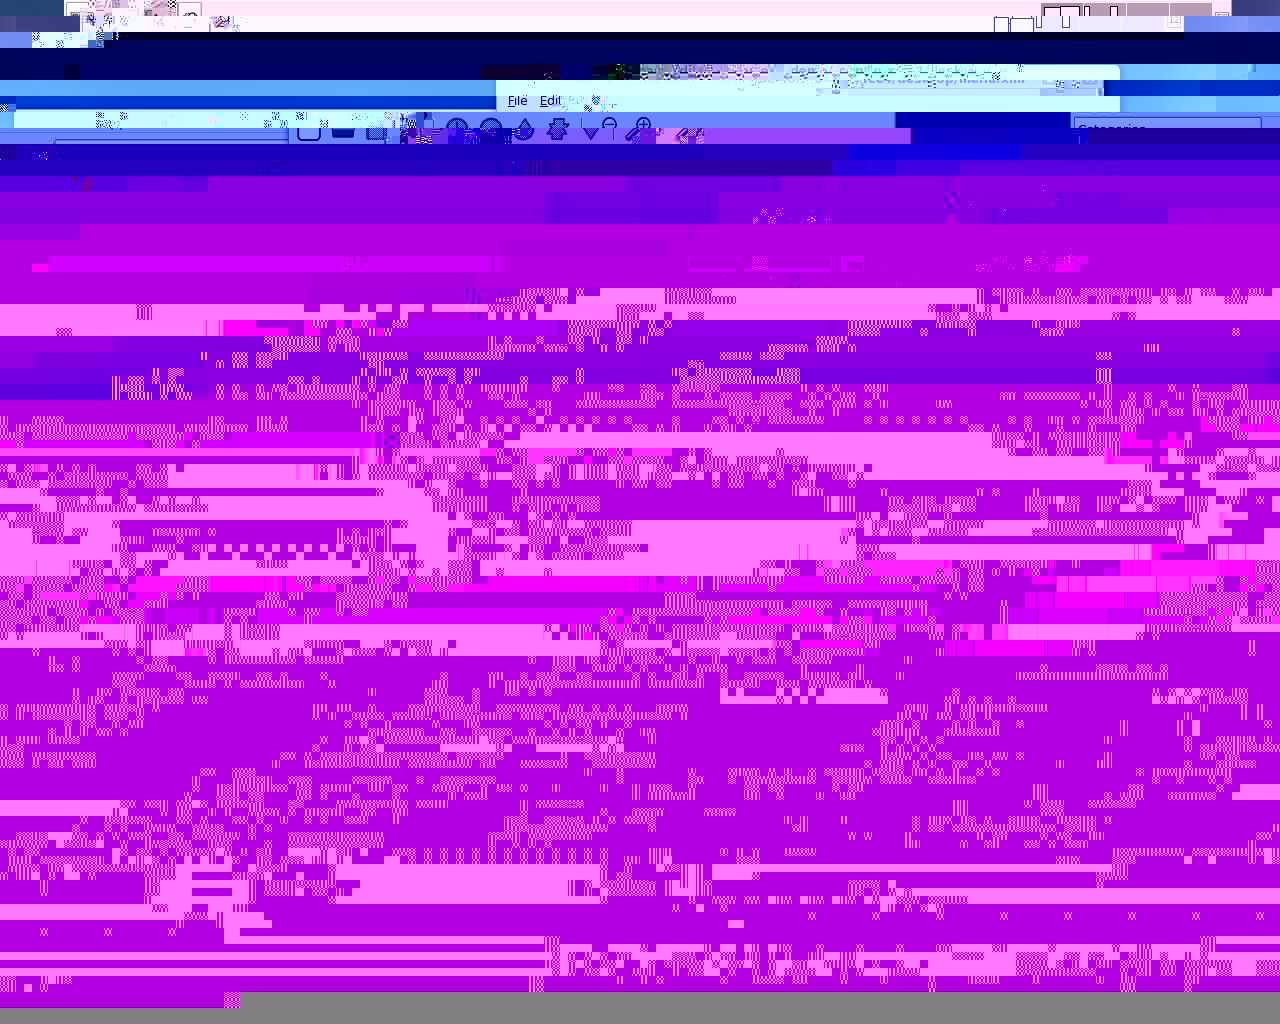
\includegraphics[height=3cm,width=4cm]{./imgs/xfce.jpg} \\ XFCE
			\end{tabular} \\
			\begin{tabular}c
		
\includegraphics[height=3cm,width=4cm]{./imgs/afterstep.jpg} \\ AfterStep 
			\end{tabular} &
			\begin{tabular}c
		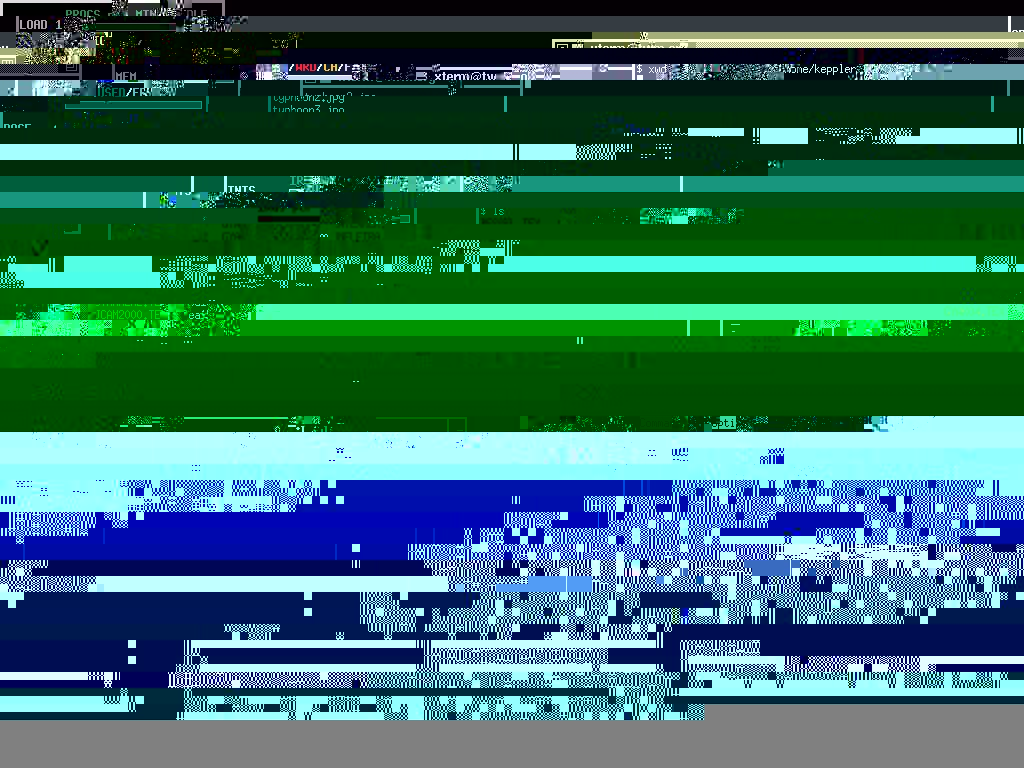
\includegraphics[height=3cm,width=4cm]{./imgs/twm.jpg} \\ TWM 
			\end{tabular}
		\end{tabular}
	\end{center}	

}


\section{Escritorio KDE}
\subsection{Presentaciones}
\frame
{
  \frametitle{La ``K'' y Konqui}
  \begin{center}
    \includegraphics[height=3cm,width=3cm]{./imgs/logo.jpg}
    \hspace{2cm}
    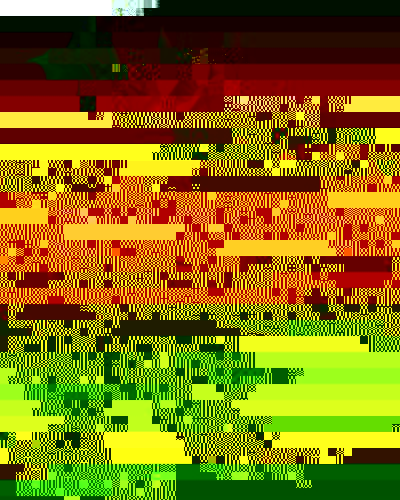
\includegraphics[height=4cm,width=3cm]{./imgs/konqui.jpg}
  \end{center}
}
\frame{
	\frametitle{Tux}
	\begin{center}
    \includegraphics[height=6cm]{./imgs/Penguin.png}
	\end{center}	
}

\subsection{Entrando al sistema}
\frame
{
  \frametitle{KDM}
  \begin{center}
    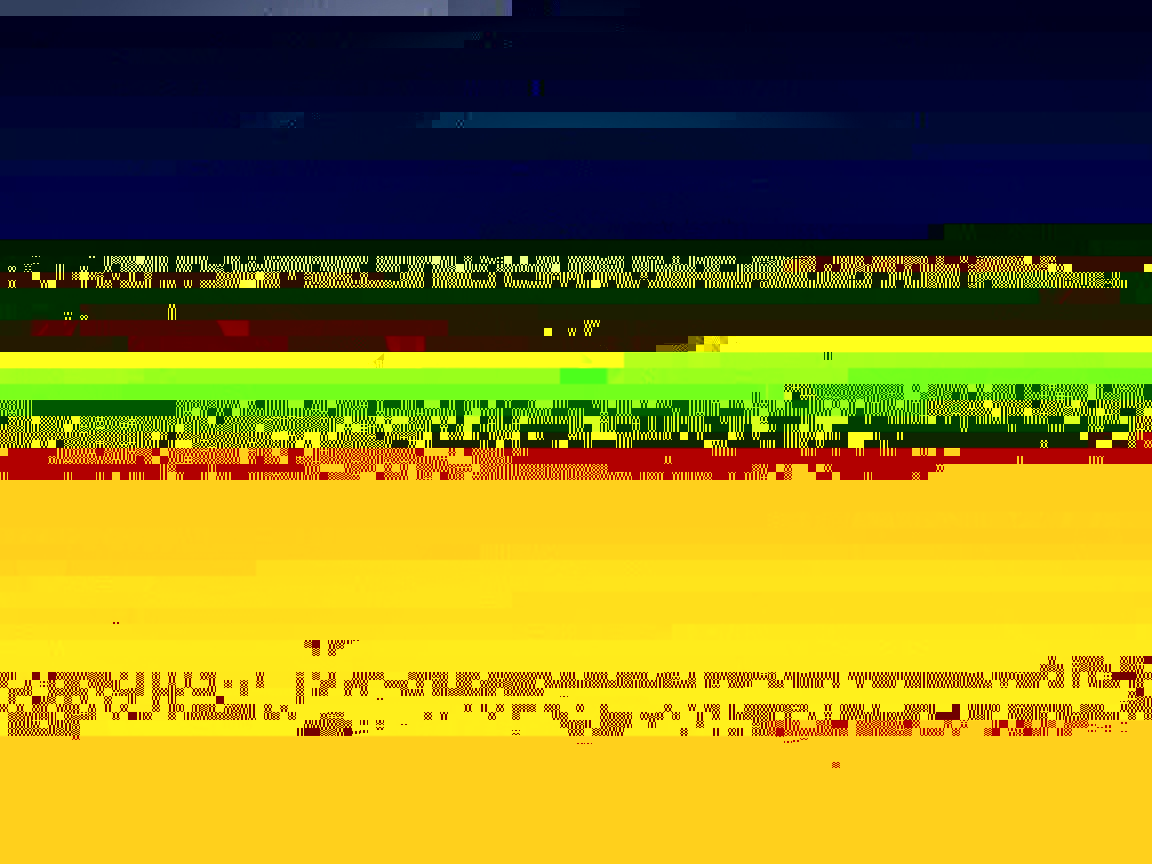
\includegraphics[height=5cm]{./imgs/kdm}
  \end{center}

}
\subsection{Aspecto Bardinux}
\frame
{
	\begin{center}
		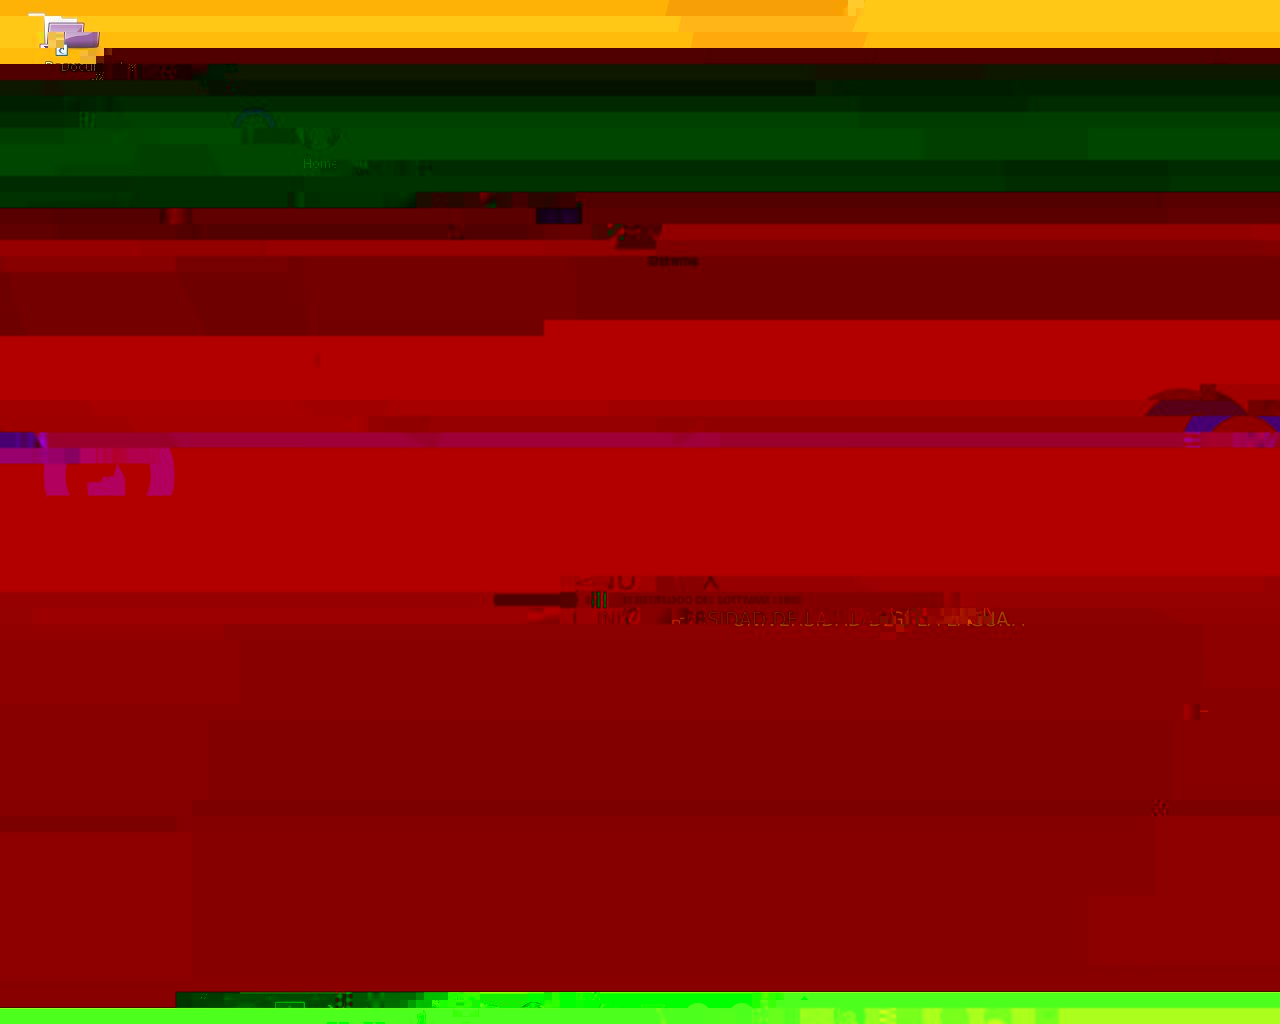
\includegraphics[width=8cm]{./imgs/kde_bardinux.jpg}
	\end{center}
}
\subsection{El kicker (la barrita de abajo)}
\frame
{
	\frametitle{El kicker}
	\begin{center}
		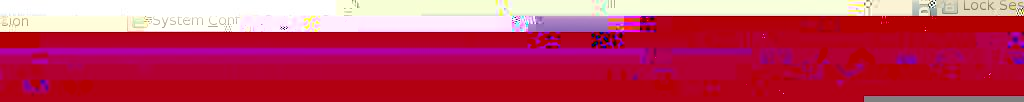
\includegraphics[height=1cm,width=10cm]{./imgs/kicker.jpg}
	\end{center}
	\begin{itemize}
		\item{El menú K}
		\item{El paginador de escritorio}
		\item{La bandeja del sistema}
	\end{itemize}
}
\frame
{
	\frametitle{Algunos Applets Más}
	\begin{itemize}
		\item<1->{Menú K}
		\item<2->{Paginador de Escritorios}
		\item<3->{Barra de tareas}
		\item<4->{Bandeja del sistema}
		\item<5->{Paginador y previsualizador del escritorio}
		\item<6->{Papelera}
		\item<7->{Klipper}
	\end{itemize}
}
\subsection{Configurar KDE}
\frame
{
	\frametitle{KControl}
	\begin{center}
		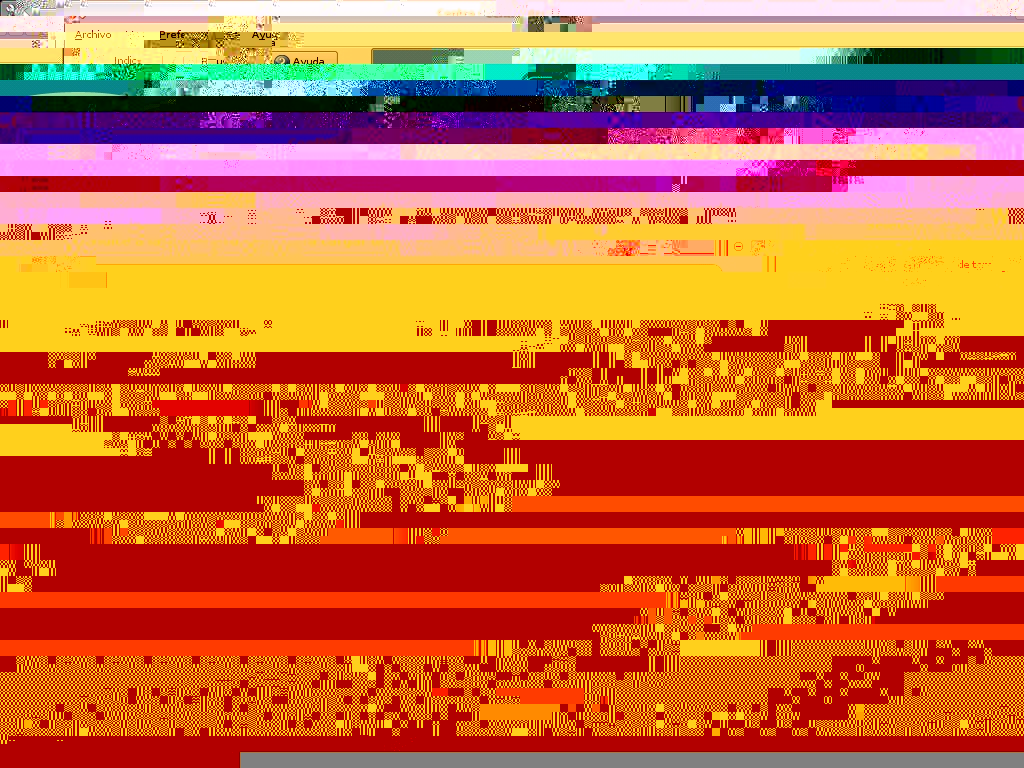
\includegraphics[height=6cm]{./imgs/kcontrol.jpg}
	\end{center}
}
\frame
{
	\frametitle{Preferencias del sistema}
	\begin{center}
		\includegraphics[height=6cm]{./imgs/pref_sistema.jpg}
	\end{center}
}
%\frame
%{
%	\large{La bandeja del sistema}
%	El reloj, amarok y varias cosas más se colocan en la bandeja del sistema
%}
\subsection{Konqueror: El .. uhmmm... esto ... }
\frame
{
	\frametitle{Konqueror: Chico para todo}
	\begin{center}
		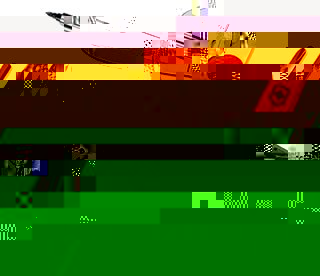
\includegraphics[height=4cm,width=4cm]{./imgs/navaja}
	\end{center}

	\begin{itemize}
		\item{Exlorador de ficheros}
		\item{Visor de pdf's, ps's}
		\item{Navegador}
	\end{itemize}
}

\subsection{Operaciones Básicas}
\frame
{
	\frametitle{Copiar, mover, cortar, pegar, dividir la pantalla}
	\begin{center}
		
\includegraphics[width=8cm]{./imgs/konqueror-file}
	\end{center}
}
\frame
{
	\frametitle{Ejecutar un programa}
	4 maneras diferentes de ejecutar un programa:
	\begin{itemize}
		\item Katapult -> Alt + Barra Espacio 
		\item Ventana ejecutar comando -> Alt + F2
		\item Click con el ratón en el icono del programa
		\item Desde una consola o shell
	\end{itemize}
}
\frame
{
	\frametitle{Asociar tipos de archivos con programas}
	\begin{center}
		
\includegraphics[height=3.5cm]{./imgs/konqueror-preferencias-general}
		
\includegraphics[height=3.5cm]{./imgs/konqueror-asociacion-mime}
	\end{center}
}


\section{KDE Conceptos Básicos Unix}
\subsection{Usuarios y grupos}
\frame
{
	\frametitle{Usuarios y grupos}
	\begin{center}
		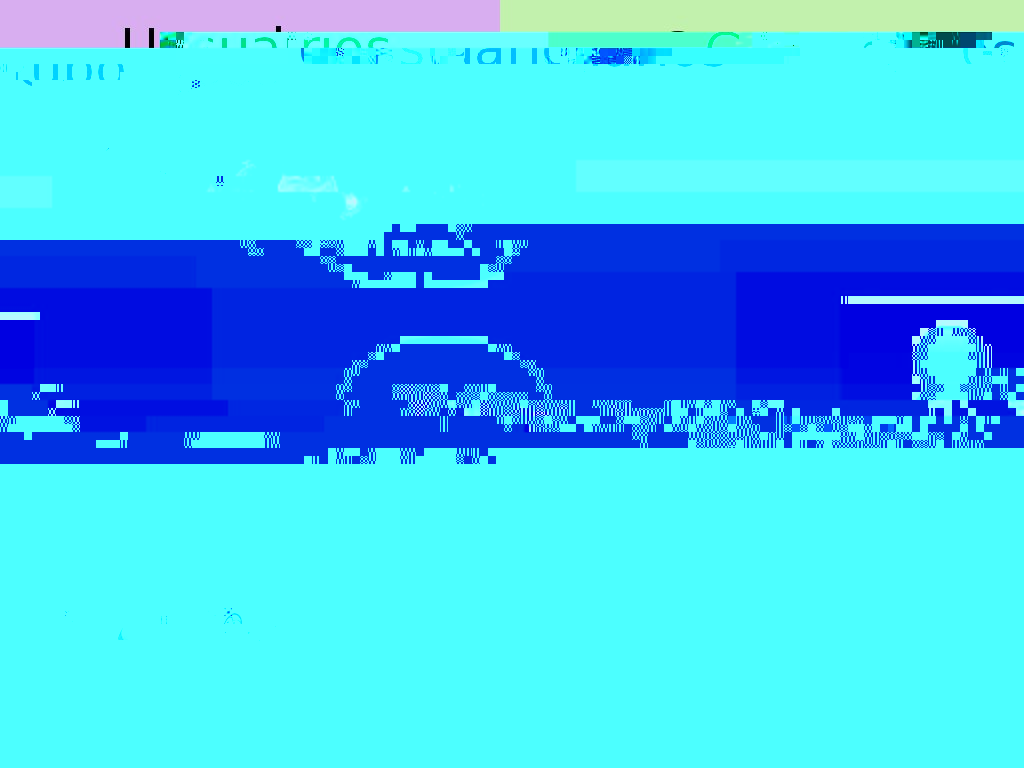
\includegraphics[width=8cm]{./imgs/usuarios-grupos}
	\end{center}
}
\subsection{Permisos en Linux}
\frame
{
	\frametitle{Permisos en linux}
	\begin{center}
		\begin{itemize}
			\item<1->{Se diferencian entre prvilegios para directorios y privilegios para ficheros}
				\begin{itemize}
					\item<2->{En ficheros: lectura, escritura y ejecución}
					\item<3->{En directorios: ver el contenidos, modificar el contenido, entrar en el directorio}
					\item<4->{Permisos especiales: +s, +t ...}
				\end{itemize}
			\item<5->{Se pueden especificar para el dueño del fichero, el grupo al que pertenece el fichero y el resto de usuarios}
		\end{itemize}
	\end{center}
}
\frame
{
	\frametitle{Modificar los privilegios de los ficheros}
	\begin{center}
		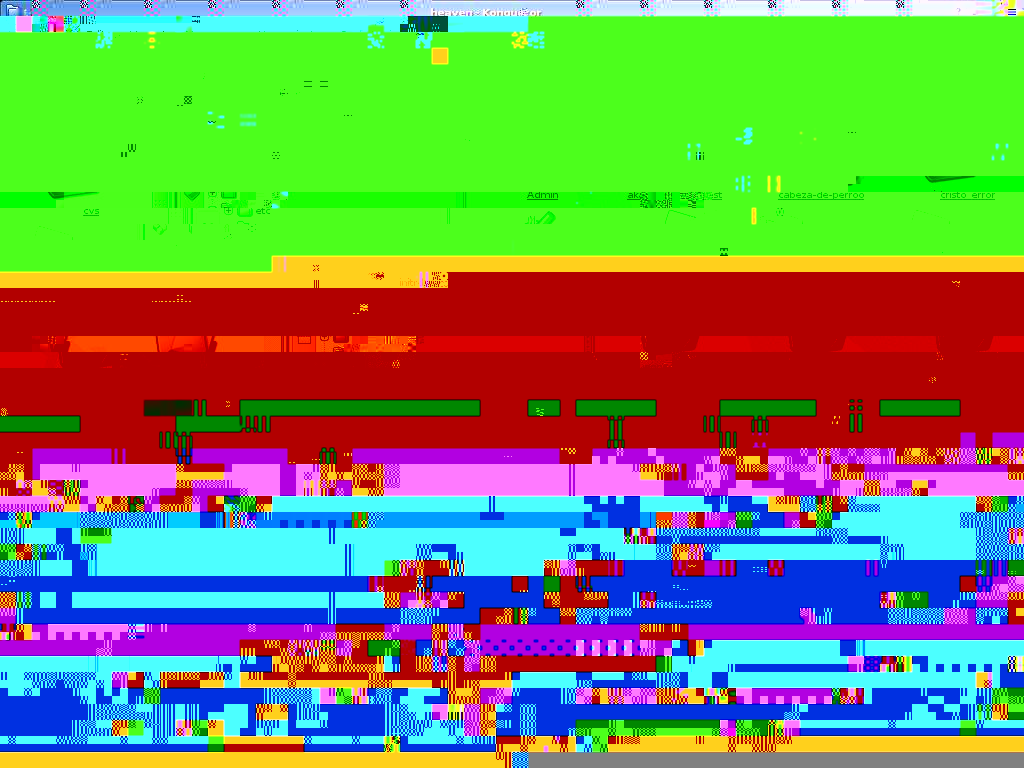
\includegraphics[height=3.5cm]{./imgs/konqueror-preferencias}
		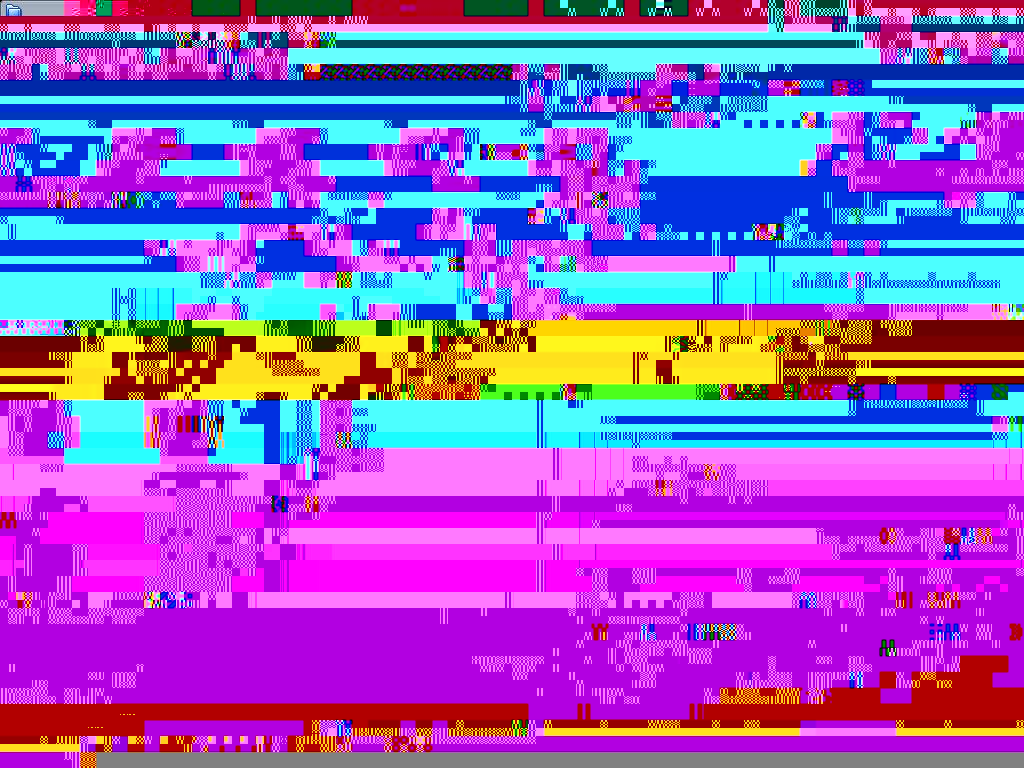
\includegraphics[height=3.5cm]{./imgs/konqueror-privilegios}
	\end{center}
}

\subsection{El árbol de directorios}
\frame
{
	\frametitle{El árbol de directorios}
	\begin{center}
		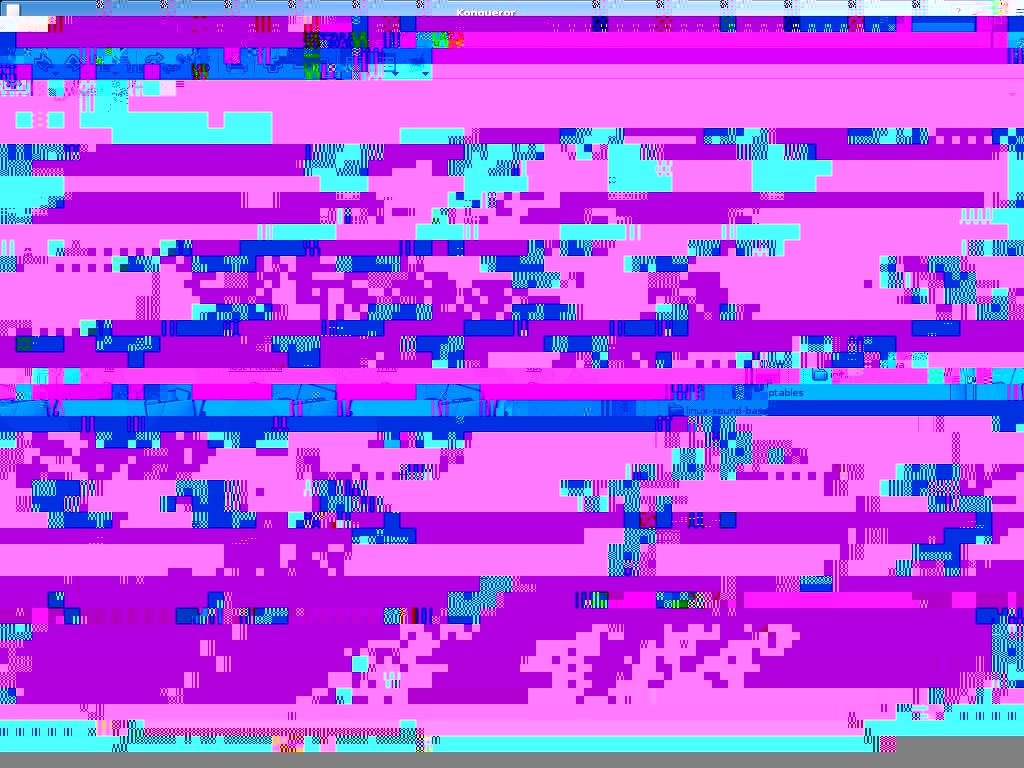
\includegraphics[height=6cm]{./imgs/konqueror-arbol}
	\end{center}
}

\section{KDE Instalación Programas}

\section{KDE Internet}
\subsection{Navegador Firefox}
\frame
{
	\begin{center}
    
\includegraphics[height=6cm]{./imgs/konqueror-gulic}
  \end{center}
}
\subsection{Chat y Clientes de Mensajería Instántanea}
\frame
{
	\frametitle{konversation, cliente de IRC}
	\begin{center}
		\includegraphics[height=6cm]{./imgs/konversation}
	\end{center}
}
\frame
{
	\frametitle{Kopete, cliente de mensajería instantánea}
	\begin{center}
		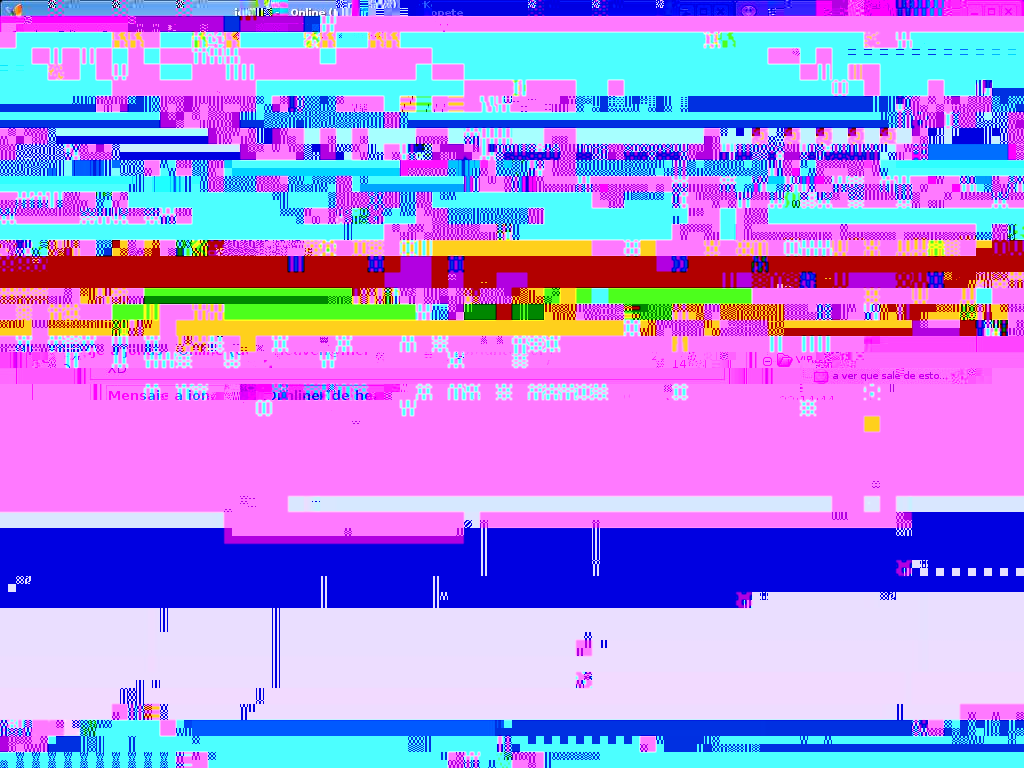
\includegraphics[height=6cm]{./imgs/kopete}
	\end{center}
}
\subsection{Cliente de correo}
\frame
{
	\frametitle{Kmail}
	\begin{center}
		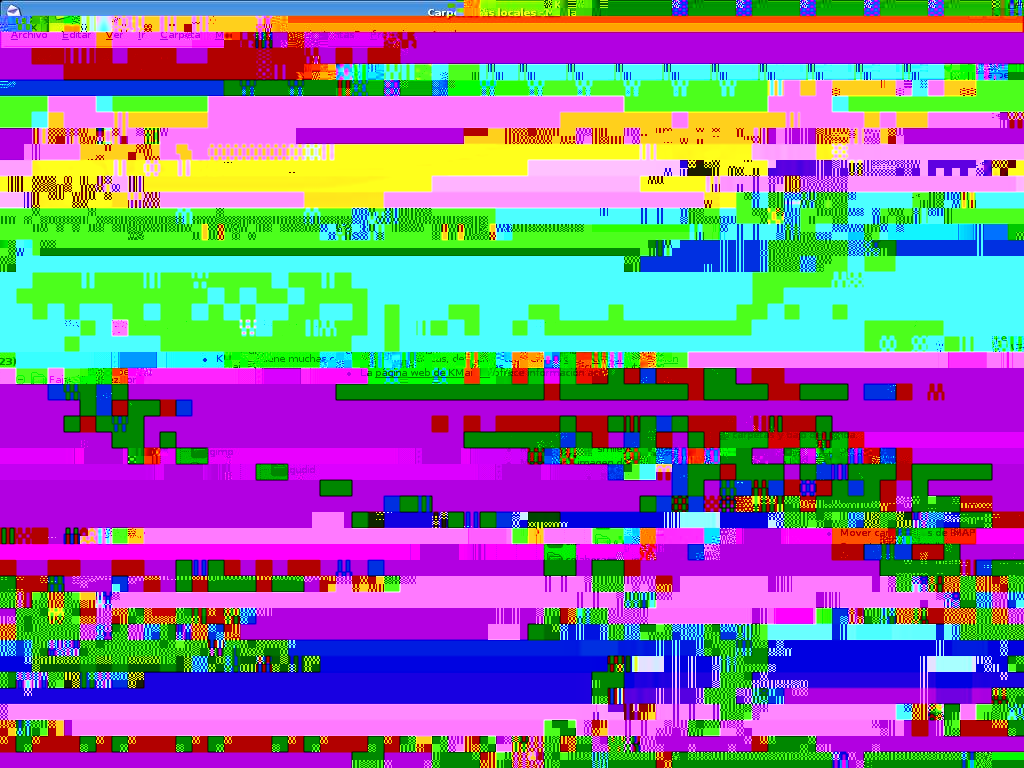
\includegraphics[height=6cm]{./imgs/kmail}
	\end{center}
}
\subsection{Gestor de Información Personal}
\frame
{
	\frametitle{Kontact}
	\begin{center}
		
\includegraphics[height=6cm]{./imgs/kontact2}
	\end{center}
}
\subsection{Agregador de noticias}
\frame
{
	\frametitle{Akregator}
	Akregator es un Agregador de noticias que soporta feeds (suministro de datos) en formato RSS y Atom.
	\begin{center}
		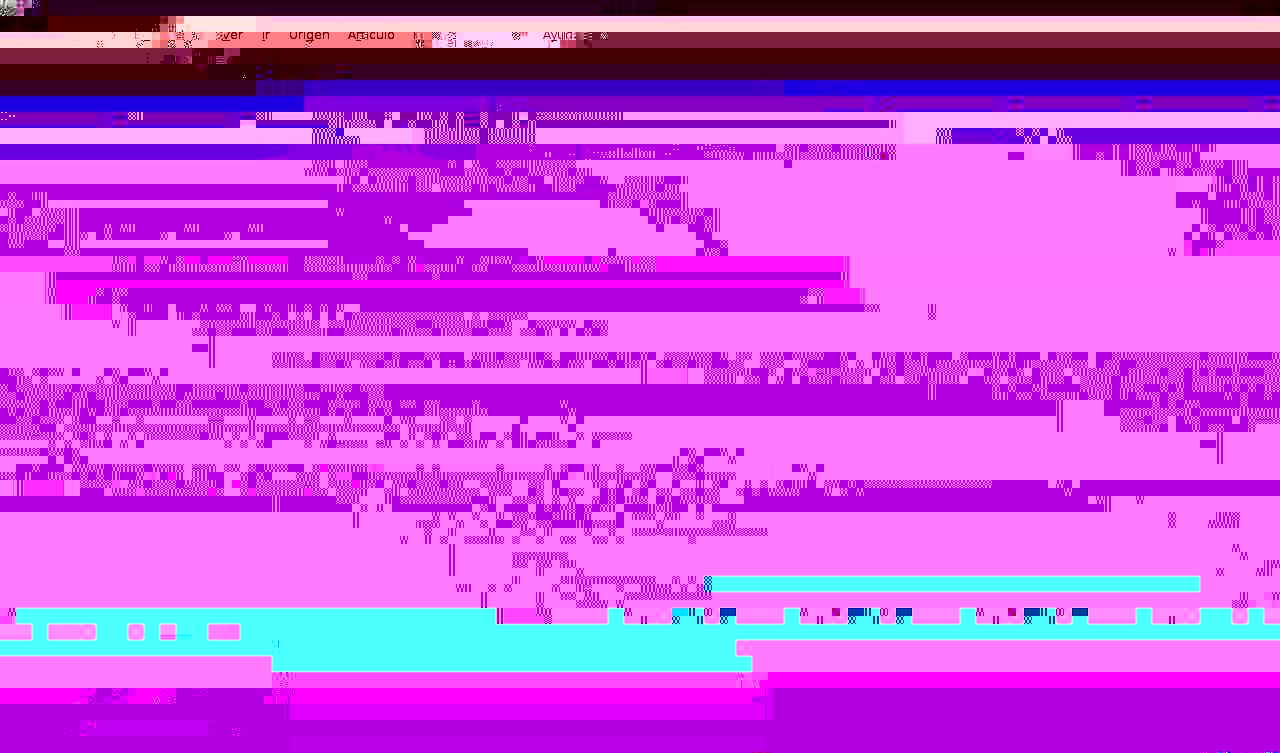
\includegraphics[height=4cm]{./imgs/akregator}
	\end{center}
}

\subsection{Internet no KDE}
\frame{
	\frametitle{Navegador Mozilla Firefox}
	\begin{center}
		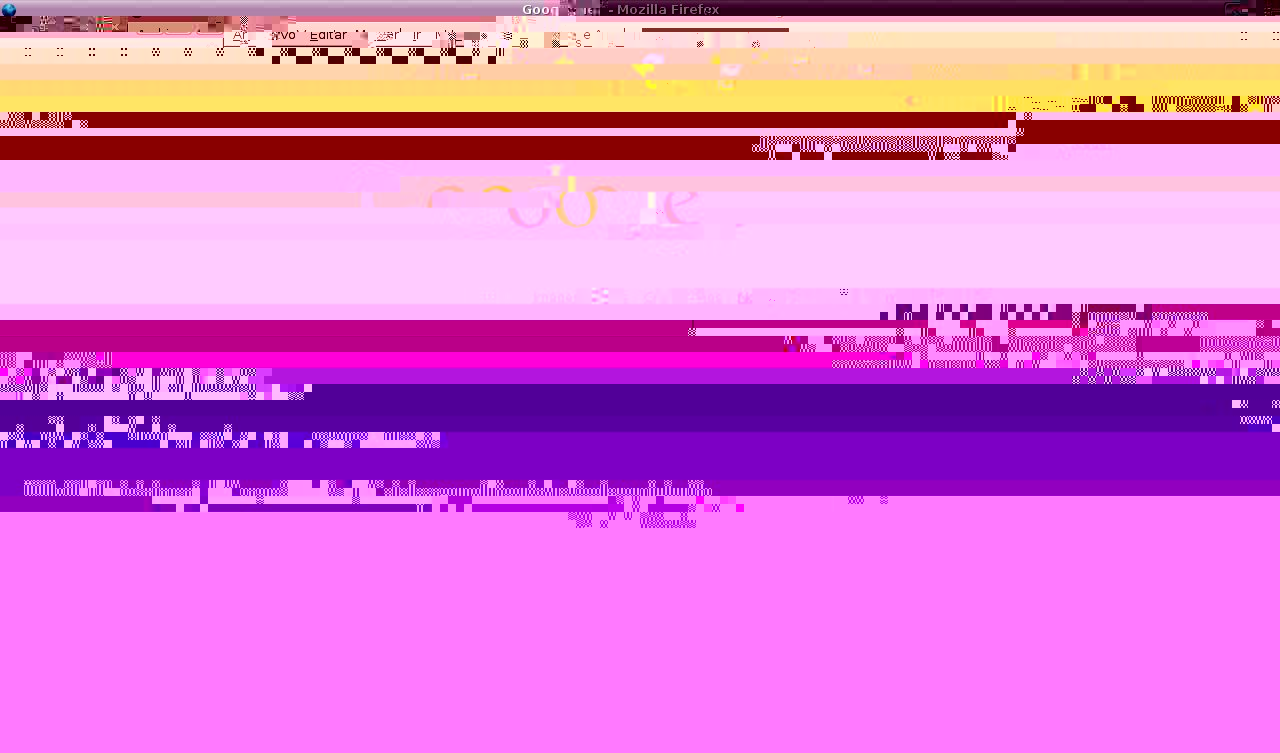
\includegraphics[height=4cm]{./imgs/firefox}
	\end{center}
	En https://addons.mozilla.org/:
	\begin{itemize}
		\item Themes: Distindos vestidos para el navegador firefox.
		\item Plugins: Acrobat Reader, Flash Player, Adblock...
		\item Extensiones: Fasterfox, ViewSourceWith, WeatherBug, Mouse Gestures...
	\end{itemize}
}
\frame
{
	\frametitle{Amsn}
	Cliente mensajería instántanea muy similar al msn para conectar con el protocolo Msn Messenger.
	\begin{center}
		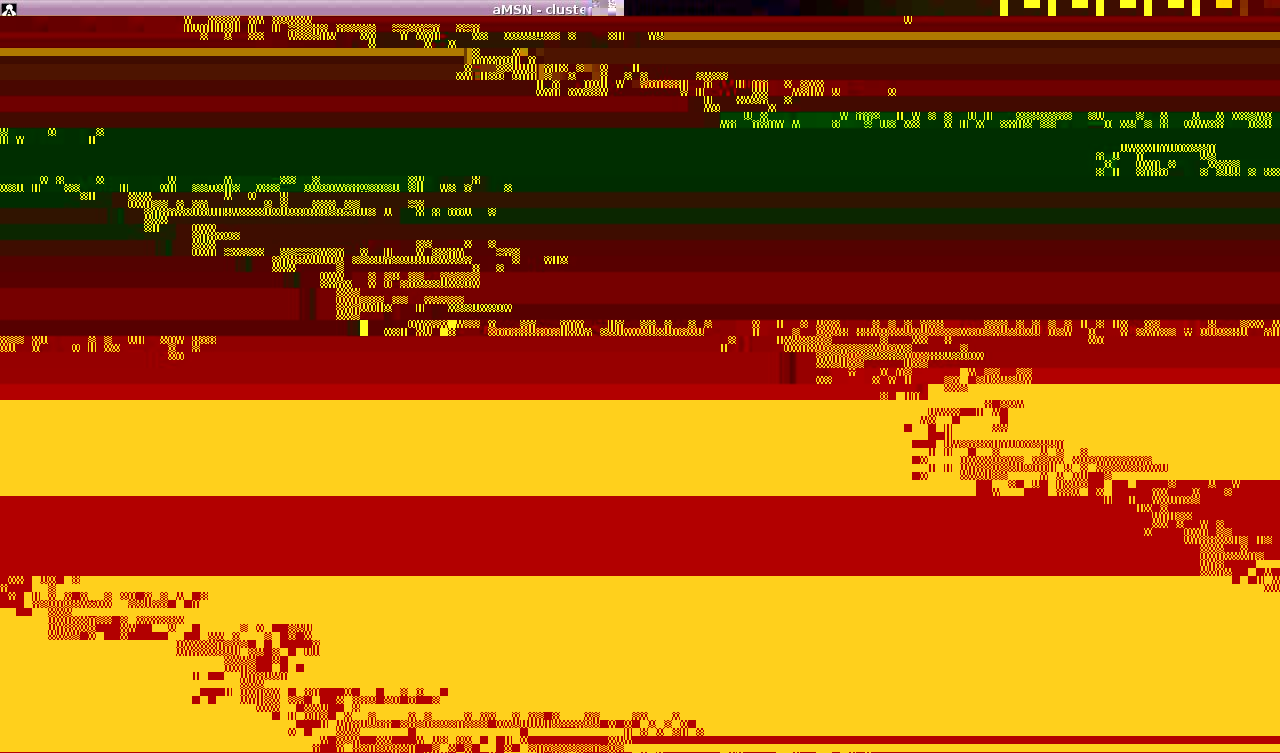
\includegraphics[height=4cm]{./imgs/amsn}
	\end{center}
}
\frame
{
	\frametitle{Amule}
	 aMule es un programa de intercambio P2P libre y multiplataforma, similar al conocido eMule que funciona tanto con la red eDonkey como con Kademlia.
	\begin{center}
		\includegraphics[height=4cm]{./imgs/amule}
	\end{center}

}

\section{KDE Multimedia}

\subsection{Grabación de CDs/DVDs}
\frame
{
	\frametitle{K3b: el kreador de CDs y DVDs}
	\begin{center}
		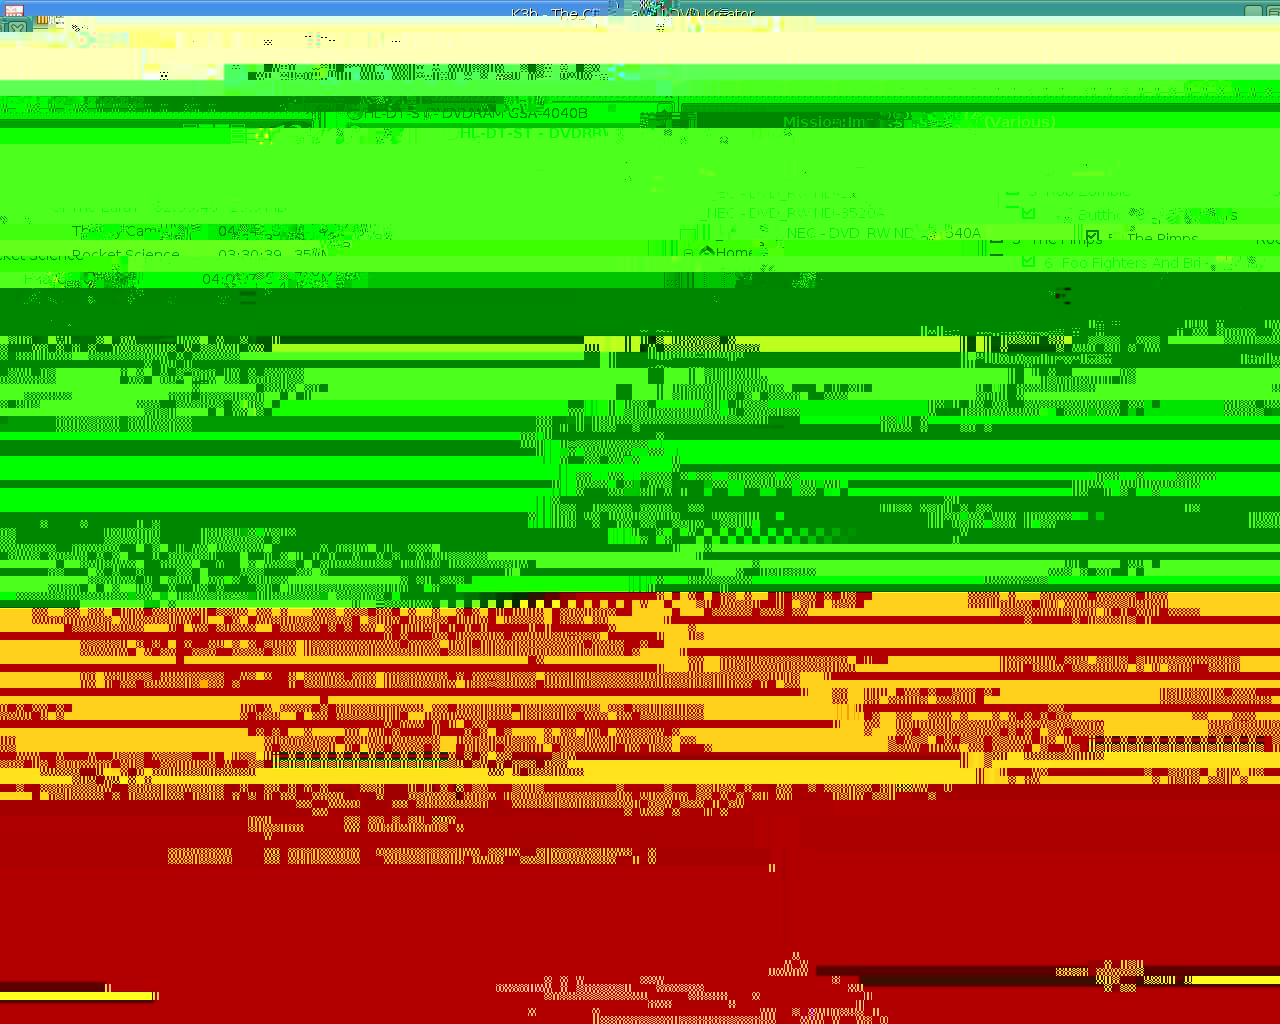
\includegraphics[height=6cm]{./imgs/k3b.jpg}
	\end{center}
}

\subsection{Reproducción de Video}
\frame
{
	\frametitle{Kaffeine}
	\begin{center}
		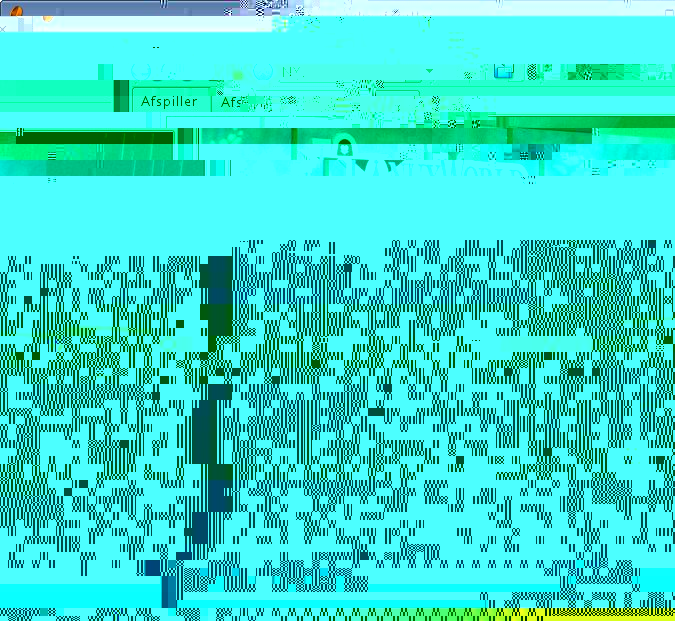
\includegraphics[height=6cm]{./imgs/kaffeine.jpg}
	\end{center}
}

\subsection{Gestión/Reproducción de Audio}
\frame
{
	\frametitle{amaroK}
	\begin{center}
		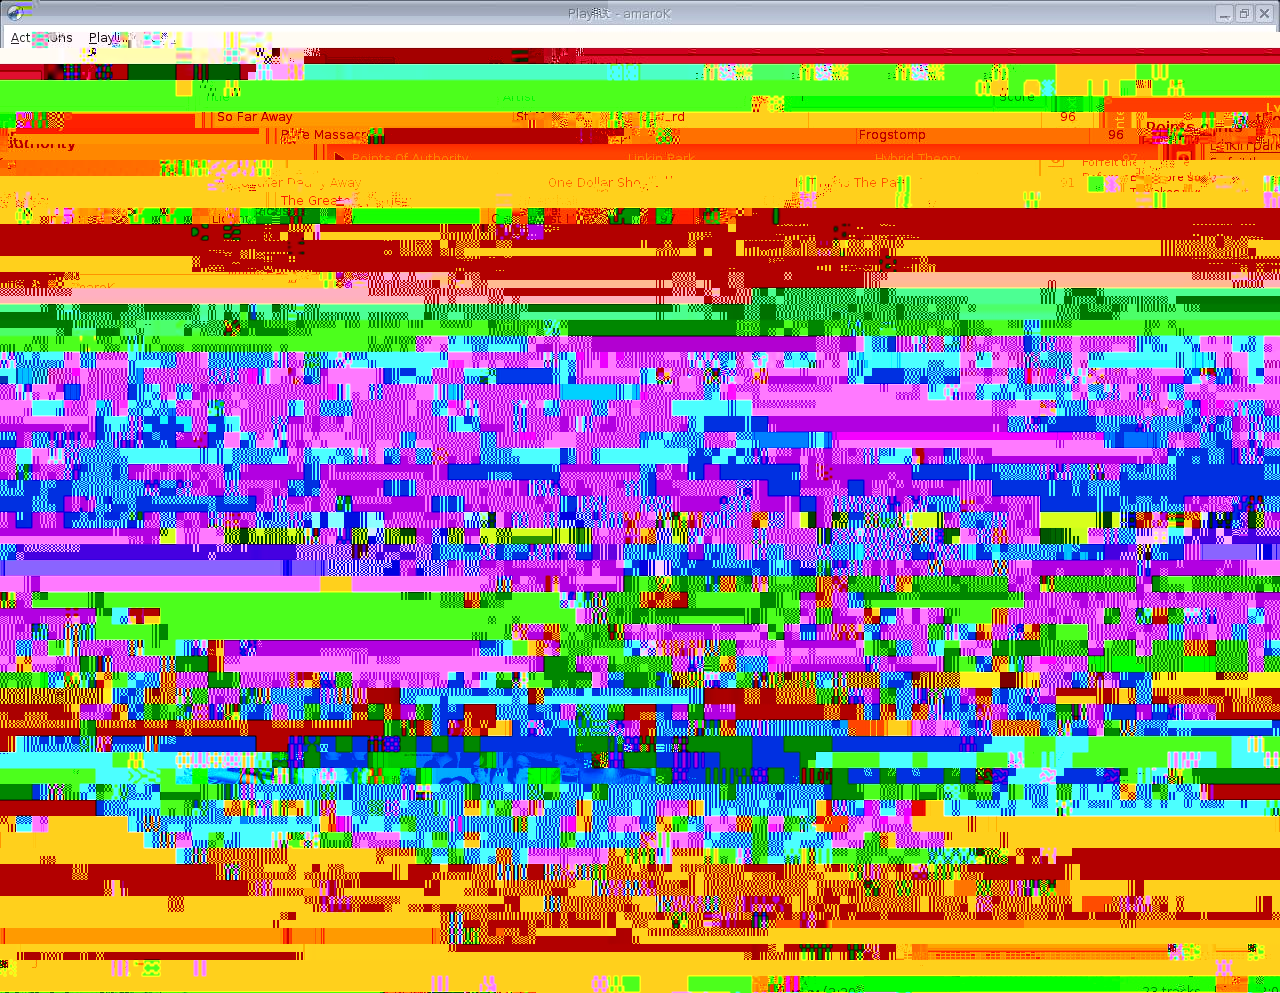
\includegraphics[height=6cm]{./imgs/amarok.jpg}
	\end{center}
}

\subsection{Edición de Video}
\frame
{
	\frametitle{Kino}
	\begin{center}
		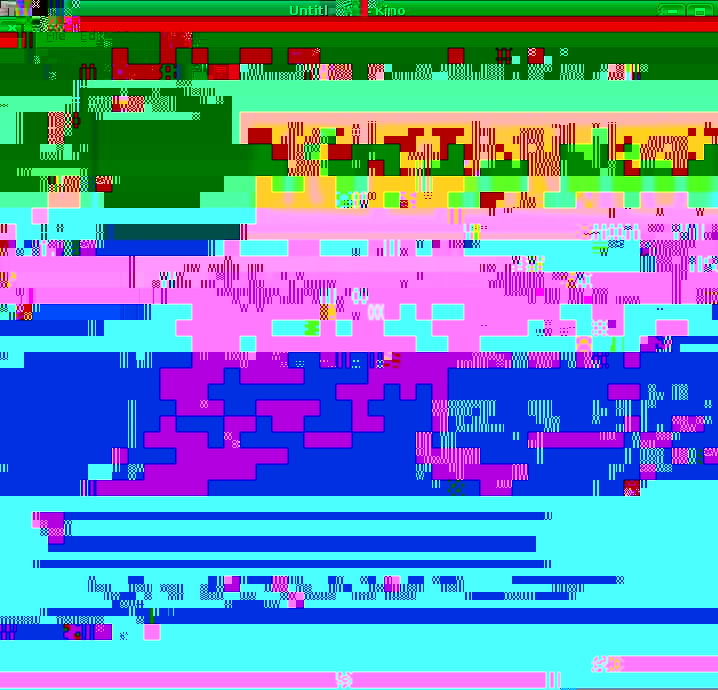
\includegraphics[height=6cm]{./imgs/kino.jpg}
	\end{center}
}

\subsection{Multimedia no KDE}
\frame
{
	\frametitle{Mplayer: Reproductor de Video}
	\begin{center}
		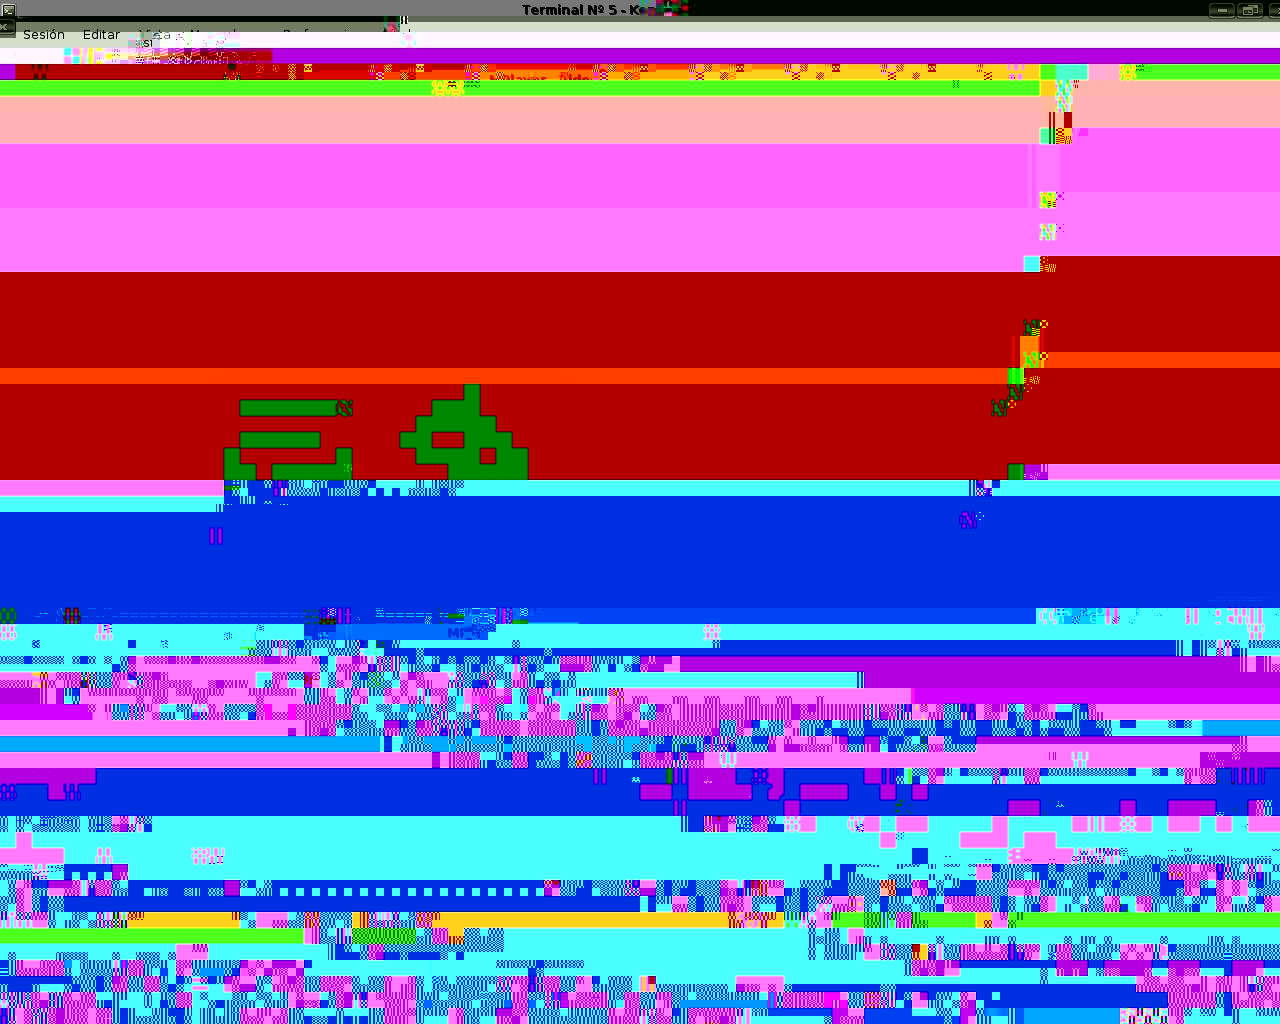
\includegraphics[height=6cm]{./imgs/mplayer.jpg}
	\end{center}
}

\frame
{
	\frametitle{Xine: Reproductor de Video}
	\begin{center}
		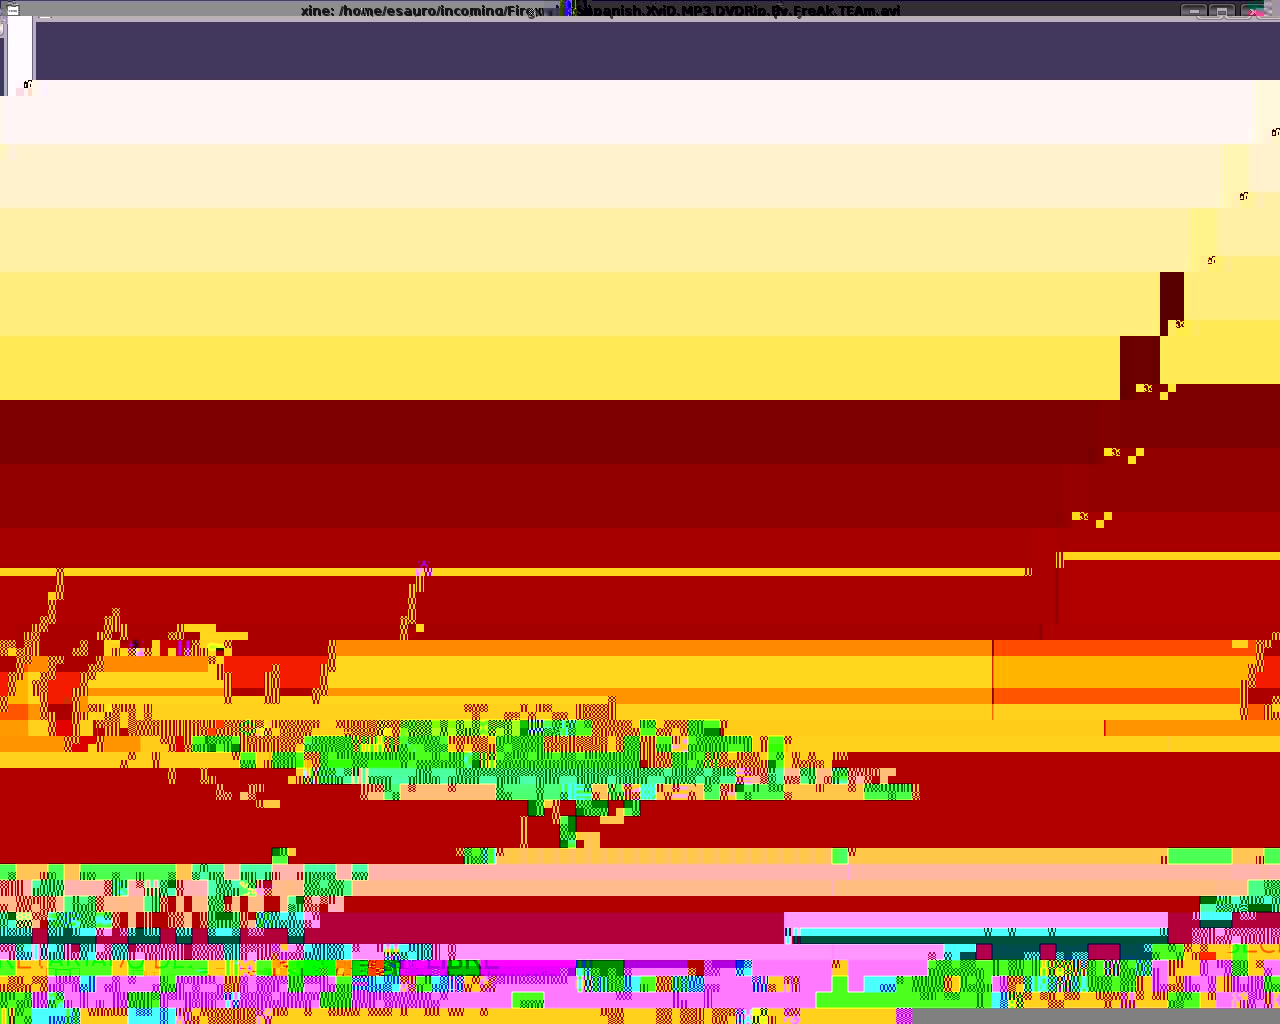
\includegraphics[height=6cm]{./imgs/xine1.jpg}
	\end{center}
}

\frame
{	
	\frametitle{XMMS: Reproductor de Audio}
	\begin{center}
		\includegraphics[height=6cm]{./imgs/xmms.jpg}
	\end{center}
}

\frame
{
	\frametitle{Audacity: Editor de Audio}
	\begin{center}
		\includegraphics[height=6cm]{./imgs/audacity-linux.png}
	\end{center}
}



\section{Para terminar...}
\subsection{URLs}
\frame
{
	\frametitle{Algunas direcciones de interés}
	\begin{itemize}
		\item<1->{www.kde.org}
		\item<2->{es.kde.org}
		\item<3->{www.kde-look.org}
		\item<4->{www.kde-apps.org}
		\item<5->{www.gulic.org}
		\item<6->{www.ssl.ull.es}
		\item<7->{cila.gulic.org}
		\item<8->{cila.ssl.ull.es}
	\end{itemize}
}
\subsection{Agradecimientos}
\frame
{
	\begin{center}
	A René Martín Rodríguez por dejarnos su presentación de KDE del año pasado que sirvió de base para esta.
	\end{center}
}
\subsection{FIN}
\frame
{
	\begin{center}
		\huge{¿Preguntas?}\\
		\pause
		\huge{Gracias por aguantarme ;-)}
	\end{center}
}
\end{document}

	
\end{document}
